\phantomsection
\section*{Chapitre 5 : Du mod\`ele \`a l'outil, le syst\`eme d'alerte pr\'ecoce}
\addcontentsline{toc}{section}{Chapitre 5 : Du mod\`ele \`a l'outil, le syst\`eme d'alerte pr\'ecoce}

\bigskip

Le chapitre~4 a d\'efini et valid\'e une approche pr\'edictive capable de
pr\'evoir l'ex\'ecution budg\'etaire avec une pr\'ecision variable mais utile selon
la cat\'egorie de d\'epense. Cependant, un mod\`ele math\'ematique, aussi bon
soit-il, ne crée de valeur que s'il peut \^etre exploit\'e par un utilisateur final.
Ce chapitre d\'ecrit la transformation de la cha\^ine pr\'edictive en un syst\`eme 
op\'erationnel : un \textbf{tableau de bord interactif} permettant aux gestionnaires
budg\'etaires de visualiser les pr\'evisions, d'identifier instantan\'ement les lignes
\`a risque, et de prendre des d\'ecisions pilot\'ees par les donn\'ees. 

L'architecture retenue s'appuie sur \textbf{Power BI}, plateforme de visualisation
retenue pour sa capacit\'e \`a produire des dashboards interactifs sans n\'ecessiter
de programmation avanc\'ee de la part des utilisateurs finaux, et sa compatibilit\'e
directe avec les fichiers Excel standard de la DPPF.

%================================================================
\phantomsection
\subsection*{5.1 \quad Cahier des charges et choix de conception}
\addcontentsline{toc}{subsection}{5.1 Cahier des charges et choix de conception}
%================================================================

\subsubsection*{5.1.1 \quad Besoins fonctionnels : vue synth\'etique et alerte cibl\'ee}

L'architecture de l'outil répond à trois besoins opérationnels distincts et
structurellement articulés~:

\begin{enumerate}
    \item \textbf{Synthèse exécutive (direction).} Un cadre dirigeant la DPPF
    doit pouvoir saisir, en quelques minutes, une compréhension synthétique~:
    combien de lignes présentent un profil à risque~? Quel montant budgétaire
    demeure exposé~? Quelle confiance opérationnelle accorder au système~?
    Cette vue s'organise autour de cinq cartes KPI stratégiques (nombre de lignes
    couvertes, dotation cumulée, taux d'exécution moyen prédit en T4, anomalies
    modérées et sévères) et de graphiques comparés réel/prédit, fournissant
    collectivement une photographie instantanée de la situation.

    \item \textbf{Analyse approfondie (gestionnaire de programme).} Un responsable
    de programme doit pouvoir circonscrire son périmètre par filtrage transversal
    sur le programme et la région, et confronter les réalisations observées (T2 au
    30~juin) aux trajectoires prédites selon deux approches modélisantes
    (\og direct \fg{} et \og rolling \fg{}). Cette interface s'appuie sur des
    \textit{slicers} dynamiques (\texttt{programme}, \texttt{region\_label}) et sur
    une table de synthèse récapitulant les prévisions T4 par catégorie budgétaire.

    \item \textbf{Détection d'anomalies et investigation ciblée (gestionnaires des
    crédits).} Les responsables des processus de paiement doivent disposer d'une
    capacité opérationnelle immédiate~: identifier quelles lignes s'écartent
    statistiquement de leurs profils historiques attendus~? Pour quelles d'entre elles
    le z-score du taux T2 descend-il sous le seuil critique de $-1{,}5$~? Cette
    interface réunit les anomalies statistiquement identifiées et les trajectoires
    historiques du taux T2 (sur six exercices) afin de contextualiser et d'interpréter
    chaque écart détecté.
\end{enumerate}

L'architecture retenue articule \textbf{deux pages} Power BI complémentaires~:
une page consolidée regroupant la synthèse exécutive et l'exploration détaillée des
lignes budgétaires (besoins 1 et 2), et une page dédiée à la détection d'anomalies
et à leur contextualisation historique (besoin 3). La navigation entre les pages est
fluide et l'ensemble des filtres positionnés sur la première page se propage
dynamiquement aux visualisations affectées.

\subsubsection*{5.1.2 \quad Choix technologiques : Power BI pour interop\'erabilit\'e}

Trois approches technologiques ont \'et\'e envisag\'ees au stade de la conception~:

\begin{itemize}
    \item \textbf{Python + Tkinter} (interface graphique de bureau)~: offrant une
    flexibilit\'e architecturale maximale, mais imposant une courbe d'apprentissage
    substantielle aux utilisateurs m\'etier.
    \item \textbf{Application web (Flask/FastAPI)}~: permettant une interactivit\'e
    riche fond\'ee sur le web, mais n\'ecessitant une infrastructure de d\'eploiement
    r\'eseau plus complexe et excluant tout fonctionnement hors connectivit\'e.
    \item \textbf{Power BI} (plateforme analytique cloud d\'edi\'ee)~: int\'egrant
    nativement le traitement de fichiers Excel, proposant une interface intuitive,
    incorporant la gestion des droits d'acc\`es, et assurant une compatibilit\'e
    structurelle totale avec l'infrastructure informatique existante de la DPPF.
\end{itemize}

Power BI a \'et\'e retenu comme solution op\'erationnelle privil\'egi\'ee, en raison
notamment du fait que cette plateforme constitue d'ores et d\'ej\`a l'infrastructure
analytique standard mobilis\'ee par le minist\`ere pour les activit\'es de pilotage et
de suivi. Les mod\`eles pr\'edictifs et les donn\'ees d'anomalies sont 
g\'en\'er\'es en Python (reproductibilit\'e, automatisation), puis import\'es en
Excel, capt\'es directement par Power BI, \'eliminant toute intervention manuelle.

%================================================================
\phantomsection
\subsection*{5.2 \quad Architecture du syst\`eme}
\addcontentsline{toc}{subsection}{5.2 Architecture du syst\`eme}
%================================================================

\subsubsection*{5.2.1 \quad Vue d'ensemble en trois composants}

\begin{figure}[H]
    \centering
    \fbox{\begin{minipage}{0.9\textwidth}
    \centering\small
    \textbf{COMPOSANT 1 : Pipeline g\'en\'eration donn\'ees (Python)}
    
    Donn\'ees TGR + morasses $\rightarrow$ pr\'etraitement + entra\^{\i}nement mod\`eles $\rightarrow$ pr\'evisions Excel
    
    Sortie : alert\_results\_2025.xlsx (130 lignes, pr\'edictions tous les mod\`eles, z-scores, risques)
    
    Sortie : historical\_recap\_2025.xlsx (5544 lignes : historique 2020--2025 par ligne)
    
    \vspace{10pt}
    
    \textbf{COMPOSANT 2 : Stockage donn\'ees (Excel)}
    
    Fichiers Excel normalis\'es : structure de table, colonnes bien d\'efinies, types coh\'erents
    
    V\'eracit\'e : agr\'egats valident exactement TGR publics
    
    \vspace{10pt}
    
    \textbf{COMPOSANT 3 : Visualisation interactif (Power BI)}
    
    Import automatique depuis Excel
    
    Deux pages stratifi\'ees~: Synth\`ese pr\'edictive et exploration (KPIs, pr\'evisions T4 par cat\'egorie, table de synth\`ese, filtres) | Anomalies (alertes + contexte historique T2)
    
    Filtres r\'eactifs : budget\_type, risk\_label, region\_label, programme
    
    \end{minipage}}
\end{figure}

\subsubsection*{5.2.2 \quad Flux de donn\'ees et architecture de causalit\'e}

L'op\'erationnalit\'e du syst\`eme repose sur un cycle de mise \`a jour
\textbf{trimestriel}, calqu\'e sur la fr\'equence de production des taux
d'ex\'ecution par la DPPF~:

\begin{enumerate}
    \item \textbf{Collecte trimestrielle} (apr\`es la cl\^oture de chaque trimestre,
    typiquement dans les deux semaines suivantes)~: la DPPF transmet aux \'equipes
    en charge des mod\`eles pr\'edictifs les taux d'ex\'ecution bruts observ\'es
    (T1, puis T2, puis T3) pour l'exercice budg\'etaire courant.
    \item \textbf{Mise \`a jour algorithmique} (dur\'ee estim\'ee~: 30 minutes)~: les mod\`eles
    pr\'ealablement calibr\'es sont r\'eex\'ecut\'es sur les donn\'ees fra\^{\i}chement re\c{c}ues.
    Les pr\'evisions T4 sont recalcul\'ees pour l'ensemble des 130 lignes, et les m\'ecanismes
    de d\'etection d'anomalies (z-scores) produisent les signaux d'alerte correspondants.
    \item \textbf{Exportation et int\'egration au tableau de bord} (dur\'ee estim\'ee~:
    5 minutes)~: les fichiers Excel cibles sont r\'eg\'en\'er\'es, puis Power BI proc\`ede
    \`a leur synchronisation automatis\'ee et rend imm\'ediatement disponibles les donn\'ees
    actualis\'ees pour consultation.
    \item \textbf{Mobilisation op\'erationnelle} (imm\'ediate)~: les gestionnaires constatent
    instantan\'ement les mises \`a jour int\'egr\'ees au tableau de bord, acc\`edent
    s\'electivement aux pages analytiques pertinentes pour leur p\'erim\`etre, et d\'eclenchent
    les investigations budg\'etaires cibl\'ees adapt\'ees aux profils ainsi r\'ev\'el\'es.
\end{enumerate}

%================================================================
\phantomsection
\subsection*{5.3 \quad Fonctionnalit\'es du tableau de bord interactif}
\addcontentsline{toc}{subsection}{5.3 Fonctionnalit\'es du tableau de bord interactif}
%================================================================

\subsubsection*{5.3.1 \quad Page 1~: synth\`ese pr\'edictive et exploration par ligne}

La premi\`ere page concentre, sur une vue unique, les indicateurs strat\'egiques
du syst\`eme et les outils d'exploration ligne par ligne. Elle r\'epond simultan\'ement
aux besoins du d\'ecideur (cinq KPI synth\'etiques en haut de page) et du gestionnaire
de programme (graphiques d\'etaill\'es par cat\'egorie, table de synth\`ese et filtres
interactifs).

\paragraph{Cartes KPI synth\'etiques~:}
Cinq indicateurs cl\'es bord\'ent la partie sup\'erieure de la page~: le nombre total
de lignes budg\'etaires couvertes (130), le montant cumul\'e des dotations (en milliards
de DH), le taux d'ex\'ecution moyen pr\'edit en T4, ainsi que le d\'ecompte des anomalies
mod\'er\'ees et s\'ev\`eres d\'etect\'ees. Cette rang\'ee fournit une photographie
instantan\'ee de l'\'etat global du syst\`eme.

\paragraph{Graphiques de pr\'evision par cat\'egorie~:}
Deux graphiques lin\'eaires juxtapos\'es comparent, ligne par ligne, le taux T4 r\'eel
au taux pr\'edit selon les deux approches \og direct \fg{} et \og rolling \fg{}.
Le premier graphique cible les d\'epenses d'\textbf{Investissement} (mod\`ele XGBoost)~;
le second couvre la cat\'egorie \textbf{Mat\'eriel} (r\'egression Ridge). Un troisi\`eme
graphique en barres agr\`ege les m\^emes m\'etriques au niveau des trois cat\'egories,
offrant une lecture comparative imm\'ediate de la qualit\'e pr\'edictive du syst\`eme.

\paragraph{Table de synth\`ese et filtres dynamiques~:}
En partie basse, une table r\'ecapitule les pr\'evisions T4 2025 par cat\'egorie
budg\'etaire (taux r\'eel observ\'e, pr\'ediction directe, pr\'ediction rolling).
Deux \textit{slicers} positionn\'es sur la droite de la page --- \texttt{programme}
et \texttt{region\_label} --- permettent un filtrage transversal en temps r\'eel~:
l'utilisateur peut, par exemple, isoler instantan\'ement les lignes du programme 301
implant\'ees dans la r\'egion Casablanca-Settat et constater l'effet sur l'ensemble
des visualisations.

% TODO: enregistrer la capture d'écran sous figures/powerbidash_page1.png puis décommenter
\begin{figure}[H]
     \centering
     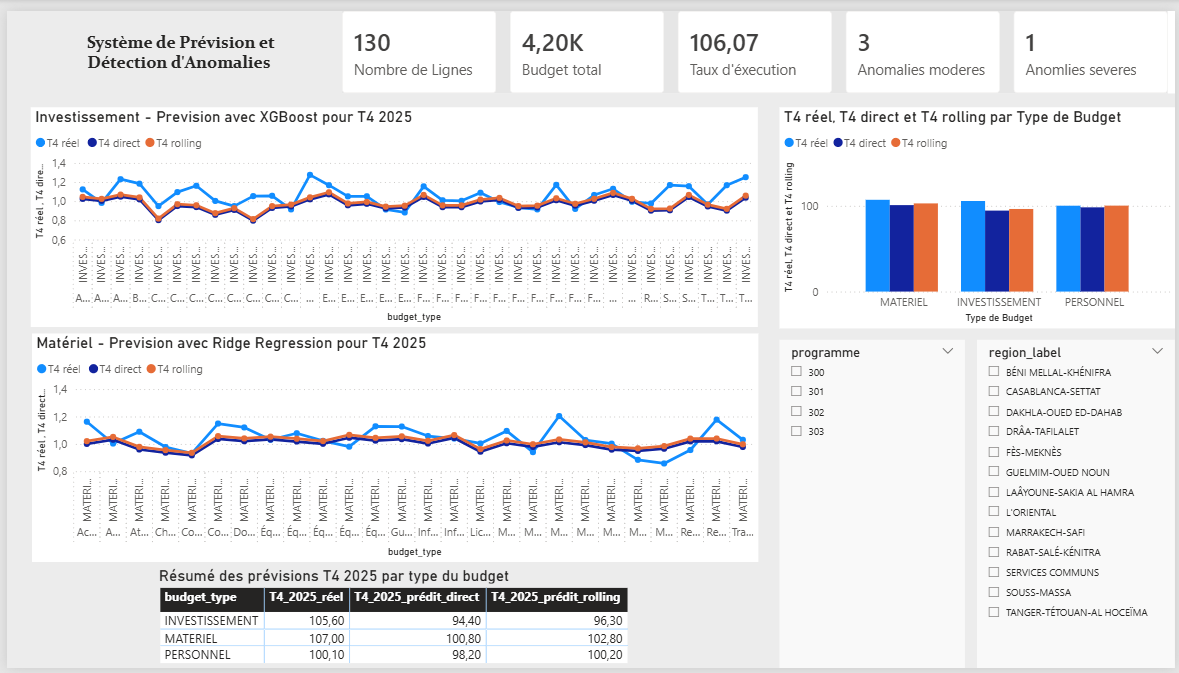
\includegraphics[width=0.98\textwidth]{figures/powerbidash_page1.png}
     \caption{\textbf{Page 1 du tableau de bord~: synth\`ese pr\'edictive et exploration par ligne.}
     La page articule cinq cartes KPI strat\'egiques (haut), deux graphiques lin\'eaires de
     pr\'evisions T4 2025 par cat\'egorie (Investissement via XGBoost, Mat\'eriel via Ridge),
     une comparaison agr\'eg\'ee r\'eel/direct/rolling par type de budget, une table de
     synth\`ese et des filtres dynamiques sur le programme et la r\'egion.}
     \label{fig:pbi_page1}
\end{figure}

\subsubsection*{5.3.2 \quad Page 2~: d\'etection d'anomalies et contexte historique}

La seconde page se consacre exclusivement aux lignes signal\'ees par le module
de d\'etection statistique. Elle articule deux composants compl\'ementaires~:
l'identification des anomalies et leur mise en perspective historique.

\paragraph{Cartes KPI restreintes aux lignes signal\'ees~:}
Les m\^emes indicateurs structurels qu'en page 1 (nombre de lignes, budget total,
anomalies mod\'er\'ees et s\'ev\`eres) sont ici recalcul\'es sur le seul p\'erim\`etre
des anomalies d\'etect\'ees, fournissant ainsi une mesure imm\'ediate de l'enjeu
financier expos\'e (33{,}82~MDH dans la configuration courante, soit quatre lignes).

\paragraph{Table des anomalies d\'etect\'ees~:}
Le tableau central liste, pour chaque ligne signal\'ee, son intitul\'e
(\texttt{ligne\_label}), sa cat\'egorie budg\'etaire, le z-score T2 calcul\'e
(quantifiant l'\'ecart \`a la trajectoire historique attendue) et le label de
s\'ev\'erit\'e associ\'e (\og Sous-ex\'ecution mod\'er\'ee \fg{} ou
\og Sous-ex\'ecution s\'ev\`ere \fg{}). Dans la configuration repr\'esent\'ee,
quatre lignes sont signal\'ees avec des z-scores compris entre $-1{,}53$ et $-2{,}01$.

\paragraph{Graphique des tendances historiques T2~:}
En partie basse, un panneau de \textit{small multiples} affiche, pour chacune
des lignes signal\'ees, la trajectoire du taux T2 sur la p\'eriode 2020--2025.
Cette mise en perspective historique permet \`a l'utilisateur de juger imm\'ediatement
le caract\`ere exceptionnel de l'\'ecart courant~: une ligne ex\'ecutant ordinairement
\`a 60\,\% au 30~juin mais ne r\'ealisant que 35\,\% en 2025 est ainsi visuellement
identifiable comme rupture par rapport \`a son propre profil. Cette contextualisation
constitue l'\'el\'ement d\'eclencheur des investigations cibl\'ees men\'ees par les
gestionnaires des cr\'edits.

% TODO: enregistrer la capture d'écran sous figures/powerbidash_page2.png puis décommenter
 \begin{figure}[H]
     \centering
     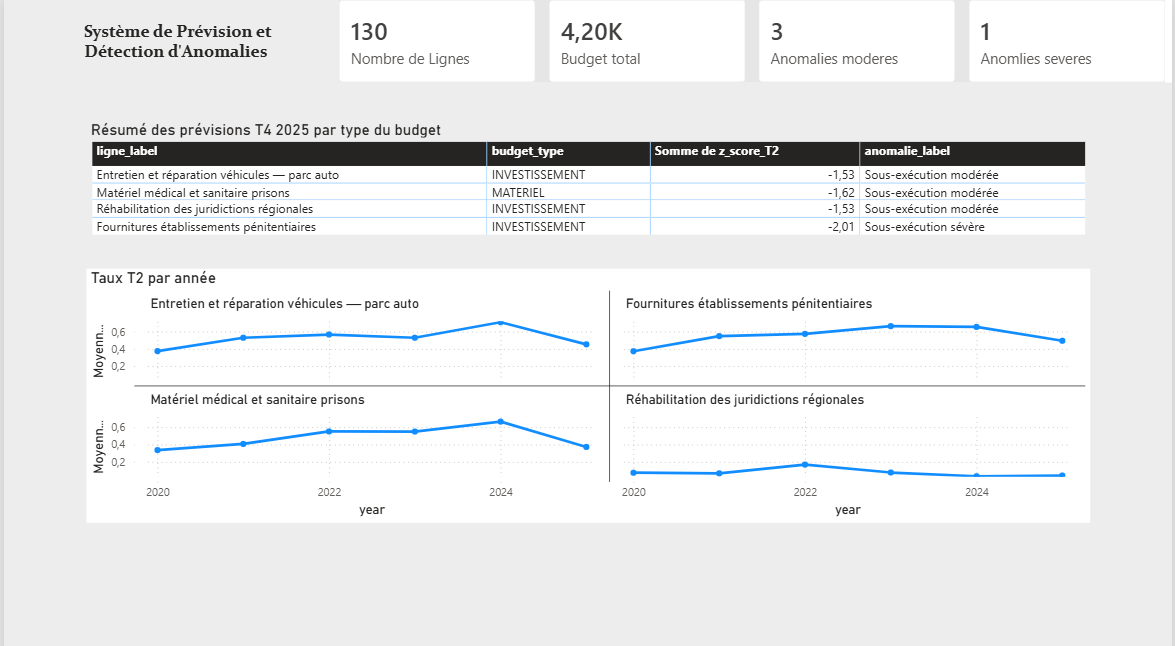
\includegraphics[width=0.98\textwidth]{figures/powerbidash_page2.png}
     \caption{\textbf{Page 2 du tableau de bord~: d\'etection d'anomalies et contexte historique.}
     La page recense les lignes signal\'ees par le module statistique (table centrale~: intitul\'e,
     cat\'egorie, z-score T2, label de s\'ev\'erit\'e) et les met en perspective via un panneau
     de \textit{small multiples} retra\c{c}ant l'\'evolution du taux T2 sur six exercices
     (2020--2025) pour chaque ligne anormale.}
     \label{fig:pbi_page2}
 \end{figure}

%================================================================
\phantomsection
\subsection*{5.4 \quad Apports op\'erationnels}
\addcontentsline{toc}{subsection}{5.4 Apports op\'erationnels et perspectives}
%================================================================

\subsubsection*{5.4.1 \quad Valeur ajout\'ee pour la DPPF}

Le système de pilotage apporte cinq avantages concrets~:

\begin{enumerate}
    \item \textbf{Alerte précoce ciblée.}

    Plutôt que de submerger les gestionnaires sous des dizaines d'indicateurs
    génériques, le système isole les quatre lignes anormales parmi 130, focalisant
    l'attention analytique sur les enjeux opérationnels réels et réduisant
    significativement le temps consacré aux investigations exploratoires.

    \item \textbf{Transparence des prévisions.}

    Les gestionnaires sont informés du fait que la prévision relative à
    l'\textsc{Investissement} présente une stabilité inférieure à celle de
    la catégorie \textsc{Personnel}, et calibrent en conséquence le degré de
    confiance accordé à chaque prédiction.

    \item \textbf{Interactivité et réduction du délai d'analyse.}

    En l'absence du tableau de bord, un responsable de programme devait commander
    un rapport manuel décrivant l'exécution ligne par ligne (un à deux jours de
    délai). Le filtrage interactif réduit cette opération à quelques dizaines
    de secondes, conférant ainsi au système une réactivité opérationnelle
    sans équivalent dans le dispositif antérieur.

    \item \textbf{Préparation simplifiée des audits et rapports trimestriels.}

    Les rapports d'exécution trimestriels, jusqu'ici produits manuellement,
    peuvent désormais être partiellement automatisés~: les exports Excel
    générés par le tableau de bord fournissent des données validées et
    directement exploitables.

    \item \textbf{Extensibilité et améliorations futures.}

    À mesure que des sources de données plus granulaires (notamment GID)
    deviendront accessibles, le système pourra être enrichi de manière
    incrémentale sans nécessiter de refonte architecturale~: seuls les
    modèles Python et les fichiers Excel intermédiaires évoluent.

\end{enumerate}

\subsubsection*{5.4.2 \quad Recommandations de déploiement et gouvernance}

L'approche reste celle adopt\'ee en Machine Learning appliqu\'e : le syst\`eme est un outil d'aide
à la décision, pas un remplaçant pour l'expertise métier. Chaque alerte doit déclencher une
investigation humaine et une validation par un responsable capable de contextualiser les
résultats, vérifier les données source, et prendre les décisions opérationnelles appropriées.
